%ब
\section{Key-Value Data Model}\label{s:key-value-data-model}
In basic terms,   the key-value data model represents data as a key-value tuple
consisting of a key,   a value and a timestamp.  A key is a unique string
commonly encoded as UTF-8.  A value is the actual data that has to be saved and
it is associated with a key that is used to retrieve the value from a key-value
database.  The value is commonly of the string data type.
This is similar to the way data is stored in a map.  A timestamp is a 64-bit
integer that records the time at which the value was inserted or updated in any
way.

Generally,   the key-value data model on cloud implements the column-oriented
approach,   which is adopted from Bigtable,   Google's cloud
\acp{DBMS}~\citep{bigtable}.
The data model explored in this section is the column-oriented key-value data model adopted by Cassandra.  This type of data model is
fundamentally different from the relational data model.  It sacrifices ACID
properties as well as normalisation in order to achieve high scalability,  
fault tolerance,   data partitioning among others.  To understand this new type
of data model and cloud \acp{DBMS} that adopt this model,   comparisons are
drawn to \acp{RDBMS} that adopt the relational model.  For this purpose a simple
example of a University database is used throughout the chapters,   where it is
assumed that students enrol into different courses.  This example is illustrated
below.

When the University database is saved in an \ac{RDBMS},   a schema will be
applied. This example assumes that the details of the students are saved in a
table called \texttt{Student} and the course details in the \texttt{Course}
table. The Student-Course relationship is maintained in a separate table called
\texttt{Enrolment} which has foreign keys for both \texttt{Student} and
\texttt{Course} tables.  This can be seen in Figure~\ref{f:RDB}. 
 
 

This shows how the University database example is deployed as a \ac{RDB}.  When
data in the University example is modelled using the column-oriented key-value
data model,   the way it is stored is different.
Although key-value \acp{DBMS} are schema-less,   column-oriented key-value
\acp{DBMS} are not entirely schema-less and hold some information about the
databases as metadata , as seen in Cassandra~\citep{datastaxDataModel}.
Such \acp{DBMS} allow applications to model the way data is organised in a
traditional \ac{RDBMS}, whilst bringing more flexibility by denormalising data
and imposing no rigid structures or schema
requirements~\citep{datastaxDataModel,BOOK,cassandra}.
Therefore,   it allows applications to add data in the way they want and change
their schema (if needed),   without adhering to a rigid schema unlike the
traditional \acp{RDBMS}.

The building blocks of column-oriented key-value \acp{DBMS} are the columns,  
the Super Columns,   the Column Family and the Key Space.  Using the
University example,   these terminologies are explained below. 
Appropriate analogies are drawn with the \ac{RDB} University,   as
seen in Figure~\ref{f:RDB}, to better understand these column-oriented key-value
concepts.  Since the focus is on Cassandra's  data model,   these concepts
are explained in the way Cassandra deploys them.  The example used
to describe the Cassandra  

\begin{landscape}
\begin{figure}[c]
	\centering
	%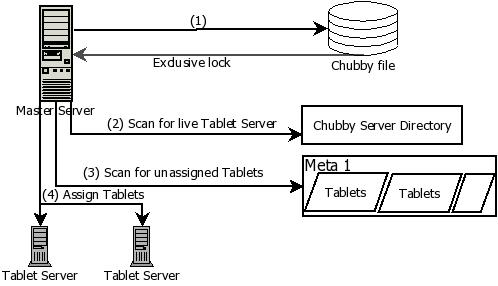
\includegraphics[width=5cm,   height=5cm]{. /figure/random. jpg}
	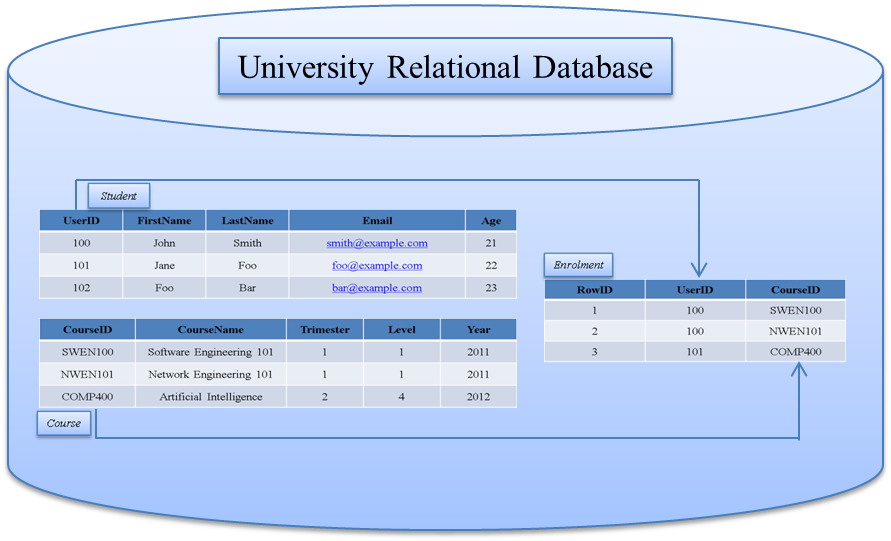
\includegraphics[width=1.4\textwidth]{./figure/Example/Relational-DB.png}
	\caption{University example as a Relational database}\label{f:RDB}
\end{figure}
\end{landscape}

\noindent data model adopts a simple and flexible schema that
allows some structure in the way data is stored. 

\todo{Fix paragraph}
As previously mentioned,  cloud \ac{NoSQL}
\acp{DBMS} are generally specialised to address specific problems like
partition-tolerance,  high availability among others and for this some trade-off
are made when these are developed.
Some of the challenges and problems present in such \acp{DBMS} are discussed in
the following section.

\subsection{Columns}
A column is the basic unit of data in this data model.  It is a
tuple containing a column name,   a value and a timestamp (Figure~\ref{f:column}). 

\begin{figure}[h]
	\centering
	%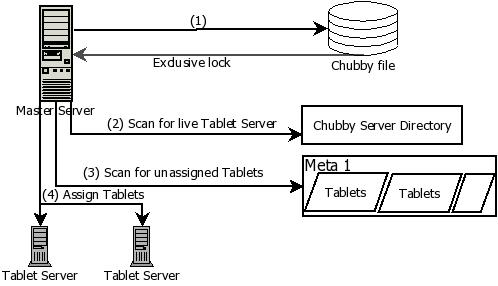
\includegraphics[width=5cm,   height=5cm]{. /figure/random. jpg}
	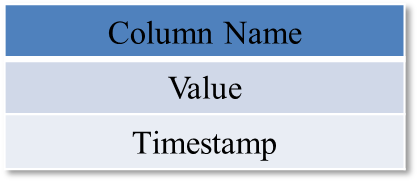
\includegraphics[width=.3\textwidth]{./figure/Example/Column.png}
	\caption{A column in Cassandra}\label{f:column}
\end{figure}

The column names are labels  and it is mandatory that a column has a name. 
Column names and values are stored as Bytes Type,   Long Type, Ascii Type,  
binary values Lexical UUID Type,   Time UUID Type or as UTF8 serialized
strings~\citep{datastaxDataModel,BOOK}.  Timstamps are used to store the time
of the latest update made to the column and are thus used for conflict resolutions.  The timestamp values are commonly stored as microseconds,   but could be in any format that the
application chooses.  However,   timestamp formats have to be consistent across
the database so that is the same format across all columns.

Cassandra allows indexes to be created on column names.  These are called
Secondary indexes and are of type \texttt{Keys} in Cassandra.  When such
secondary indexes are used,   efficient queries can be specified using equality
predicates,   and can be made on ranges of columns too.  The latter ones are
called range queries.

A column name can be considered analogous to an attribute name in a table in any
traditional \ac{RDBMS}.  To illustrate this analogy,
Figures~\ref{f:column-FirstName} and~\ref{f:RDB-User} show the differences
between the representation of values in \texttt{Student} in Cassandra and in an
\ac{RDBMS}.
It can be seen from these figures that a column in the column-oriented key-value
data model is similar to a single value in a row of a relational table.  For
example,   the data '\texttt{John}' in the relational table \texttt{Student} can
be considered equivalent to a single column in Cassandra.

\begin{figure}[H]
	\newcommand{\W}{.24\textwidth}
	\centering
	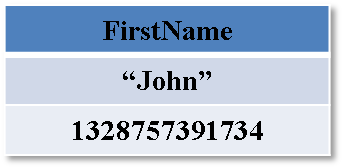
\includegraphics[width=\W]{./figure/Example/Column_FirstName.png}
	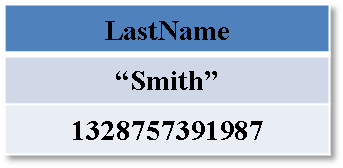
\includegraphics[width=\W]{./figure/Example/Column_LastName.png}
	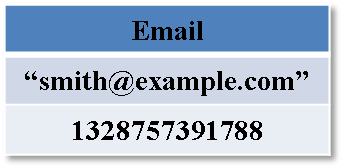
\includegraphics[width=\W]{./figure/Example/Column_Email.png}
	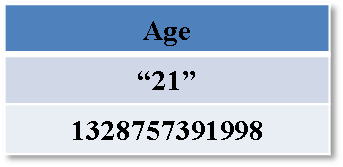
\includegraphics[width=\W]{./figure/Example/Column_Age.png}
	\caption{Columns in Cassandra}\label{f:column-FirstName}
\end{figure}

\begin{figure}[H]
	\centering
	%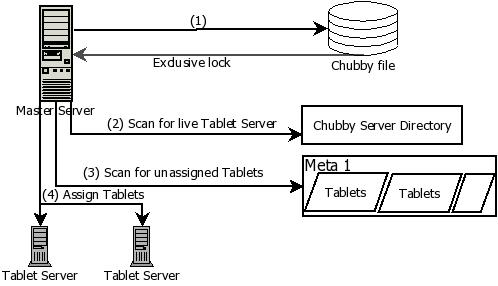
\includegraphics[width=5cm,   height=5cm]{. /figure/random. jpg}
	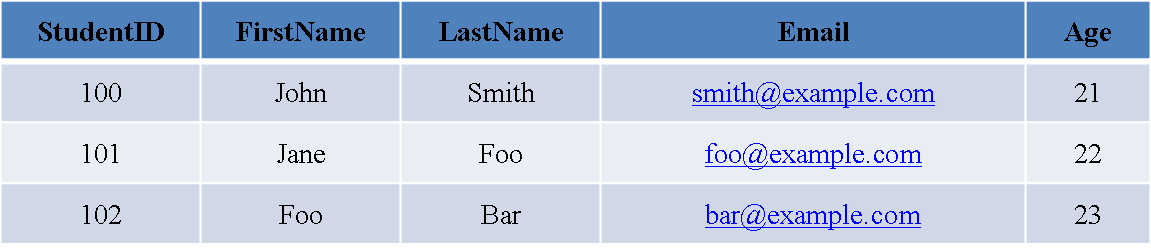
\includegraphics[width=1\textwidth]{./figure/Example/RelationalTable_User.png}
	\caption{Relational Table - Student}\label{f:RDB-User}
\end{figure}

The JSON notation for  columns in Cassandra is shown in Figure~\ref{f:column-JSON}. 

\begin{figure}[H]
	\centering
	%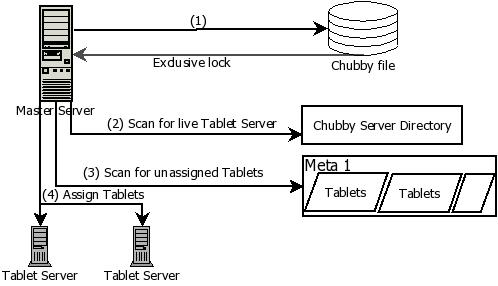
\includegraphics[width=5cm,   height=5cm]{. /figure/random. jpg}
	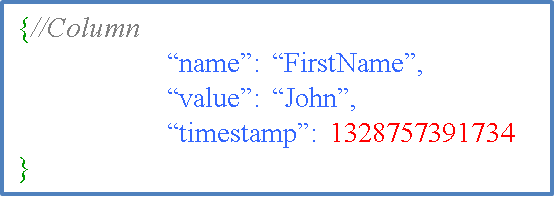
\includegraphics[width=.5\textwidth]{./figure/Example/Column_JSON.png}
	\caption{JSON notation for a column}\label{f:column-JSON}
\end{figure}
% 
% Alternatively,   applications can also use column names to store values.  This is
% possible since it is not required that columns always have values and
% since column names are byte arrays,   applications can store any kind of
% values in it. 
\subsection{SuperColumns}
A super column is a different kind of a column where the
values are an array of regular columns (Figure~\ref{f:supercolumn}).  It consists of a super
column name and an ordered map of columns.  The columns within the values of a
super column are grouped together using a common look-up value,   which is
commonly referred to as the \texttt{RowKey}.  In other words,   a super column is a
nested key-value pair of columns.  The outer key-value pair forms the super column while the inner
nested key-value pairs are the columns.  Unlike regular columns,   super columns do
not have timestamps for its key-value pairs.  

\begin{figure}[H]
	\centering
	%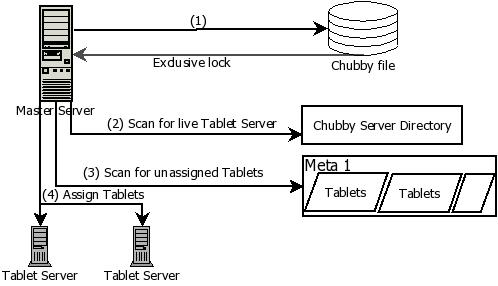
\includegraphics[width=5cm,   height=5cm]{. /figure/random. jpg}
	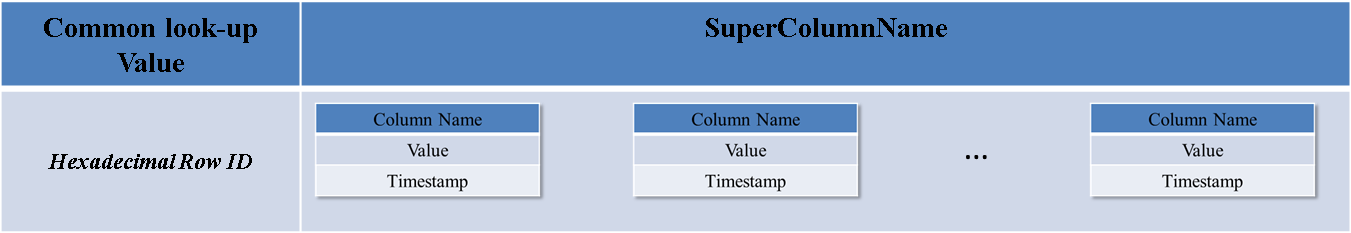
\includegraphics[width=\textwidth]{./figure/Example/SuperColumn.png}
	\caption{A Super Column }\label{f:supercolumn}
\end{figure}

A super column can be considered roughly similar to a whole record in a
relational table in an \ac{RDB}. For example,   the super column for a
student,   as seen in Figure~\ref{f:supercolumn-John},   is analogous to a single
record in the relational table \texttt{Student} (Figure~\ref{f:RDB-User}). 

\begin{figure}[H]
	\centering
	%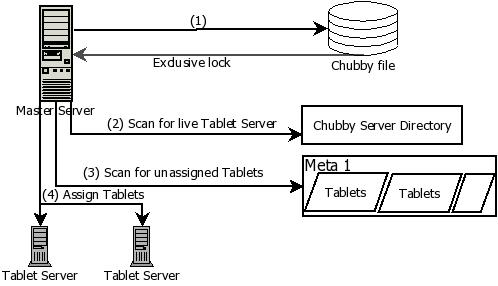
\includegraphics[width=5cm,   height=5cm]{. /figure/random. jpg}
	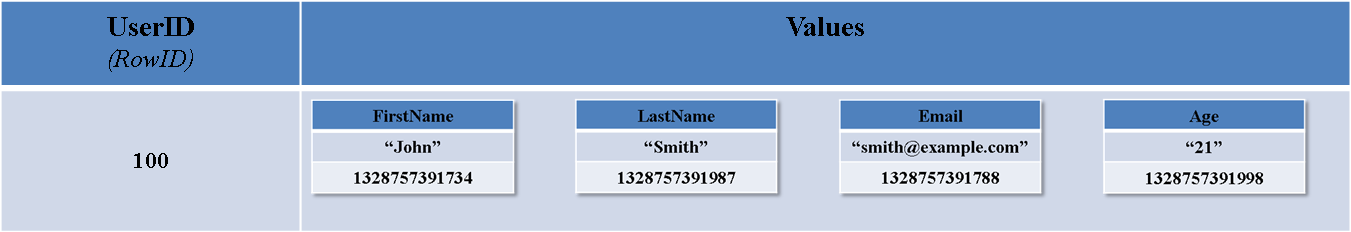
\includegraphics[width=\textwidth]{./figure/Example/SuperColumn_John.png}
	\caption{A Super Column for Student '\texttt{John}' in
	Cassandra}\label{f:supercolumn-John}
\end{figure}

\newpage

The JSON notation for a super column is shown in Figure~\ref{f:supercolumn-JSON}. 


\begin{figure}[H]
	\centering
	%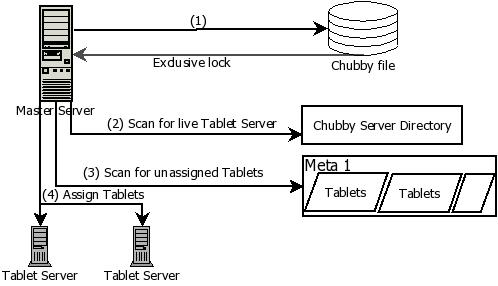
\includegraphics[width=5cm,   height=5cm]{. /figure/random. jpg}
	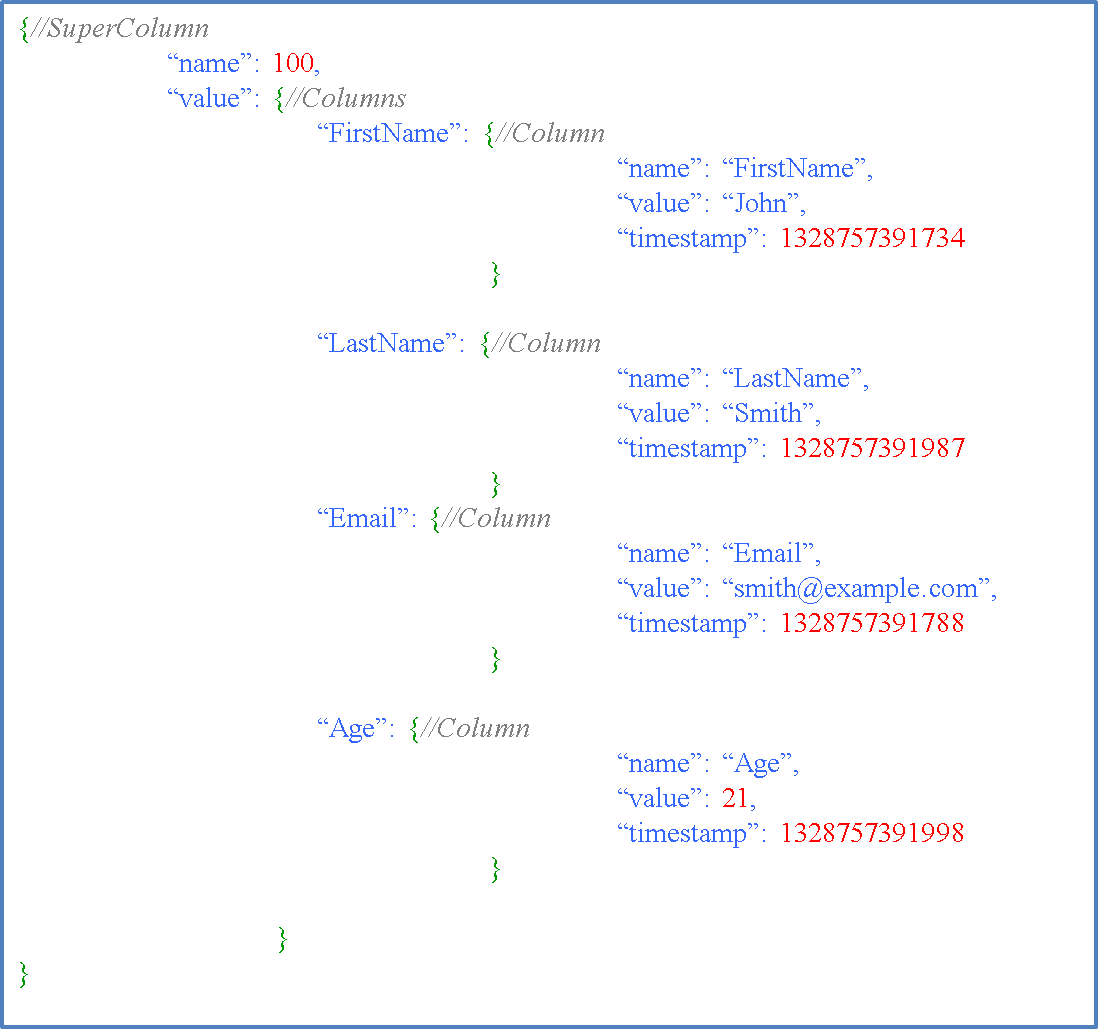
\includegraphics[width=.9\textwidth]{./figure/Example/JSON_SuperColumn_John.png}
	\caption{JSON notation for a super column}\label{f:supercolumn-JSON}
\end{figure}


\subsection{ColumnFamily}
 A column family contains columns or super columns that are
grouped together using a unique row key.  It is a set of key-value
pairs,   where the key is the row key and the value is a map of column names
(Figure~\ref{f:columnfamily}).  The row key groups the columns together,   just as
in super columns. 

\begin{figure}[H]
	\centering
	%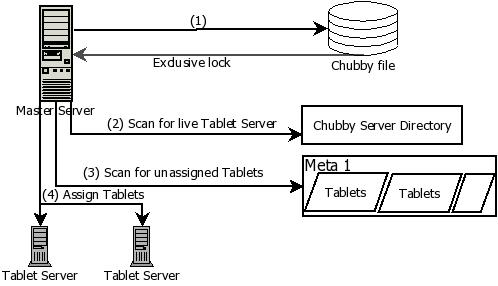
\includegraphics[width=5cm,   height=5cm]{. /figure/random. jpg}
	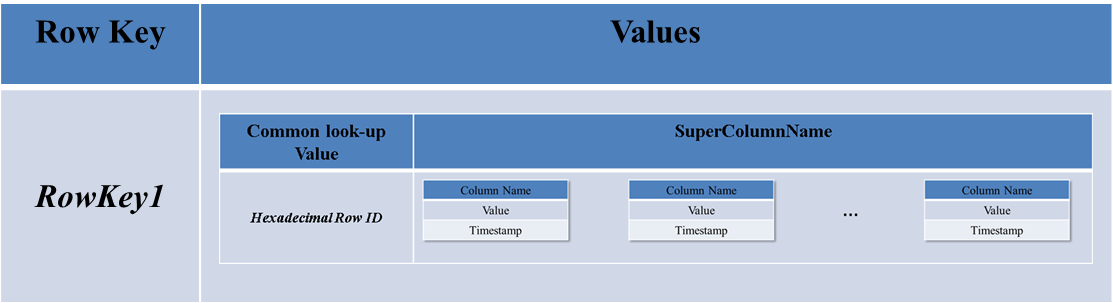
\includegraphics[width=\textwidth]{./figure/Example/ColumnFamily.png}
	\caption{Column Family in Cassandra}\label{f:columnfamily}
\end{figure}

Applications can define column families and metadata about the columns. 
It is commonly practised to have columns that are related or accessed
together to be grouped in the same column family.  Column families require that
some attributes are always defined,   like name,   column type and others.  It
also has optional attributes that can be defined if the application requires so.
 Some of the optional attributes are number of keys cached,   comments,   read
repairs,   column metadata among others.

Column families can have rows %to have relatively a definite number of columns.
that are identified by their unique row keys.  This is similar to a table in an
\ac{RDB}, as seen for table \texttt{Student} in Figure~\ref{f:RDB-User},   where
every row in the table has the same number of columns and primary keys are used
to identify a row.  An example of a column family is shown in
Figure~\ref{f:columnfamilyUSER}.
Unlike relational tables in an \ac{RDB},   column families do not require all
the rows to define the same number of columns~\citep{datastaxDataModel,BOOK}.

\begin{figure}[h]
	\centering
	%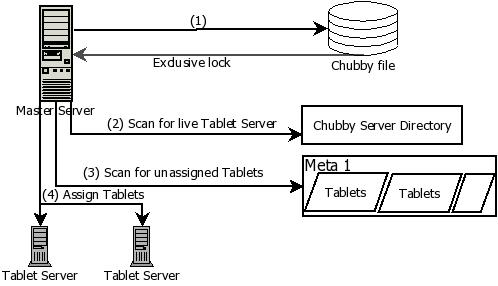
\includegraphics[width=5cm,   height=5cm]{. /figure/random. jpg}
	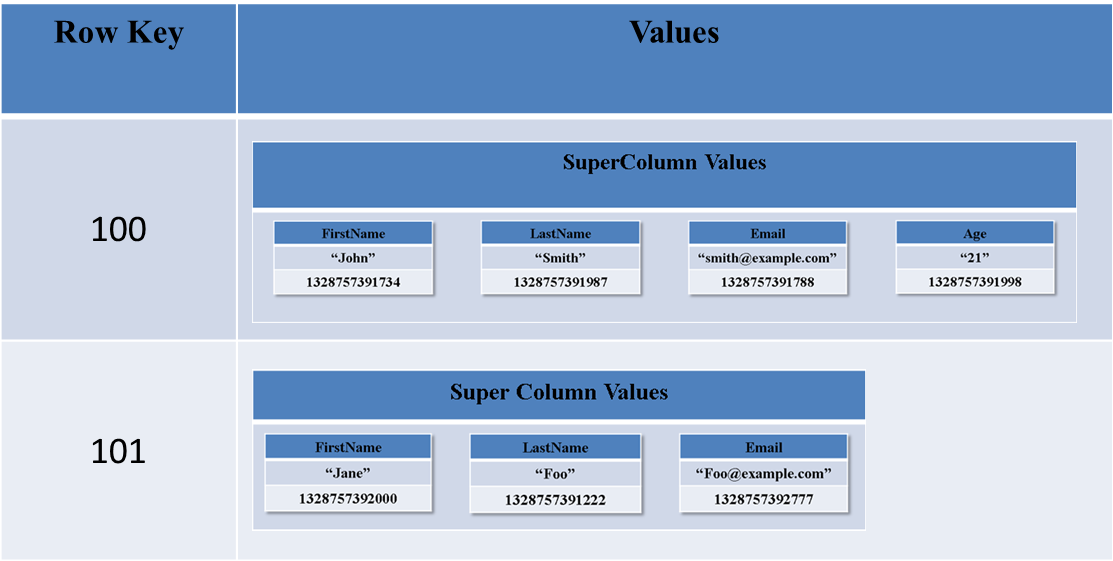
\includegraphics[width=\textwidth]{./figure/Example/ColumnFamily-User-DiffColumns.png}
	\caption{Column Family \texttt{User} in Cassandra}\label{f:columnfamilyUSER}
\end{figure}

The JSON notation for a single row of a column family in Cassandra is
shown in Figure~\ref{f:columnfamilyJSON} 

\begin{figure}[h]
	\centering
	%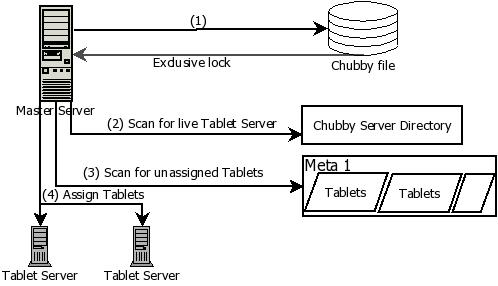
\includegraphics[width=5cm,   height=5cm]{. /figure/random. jpg}
	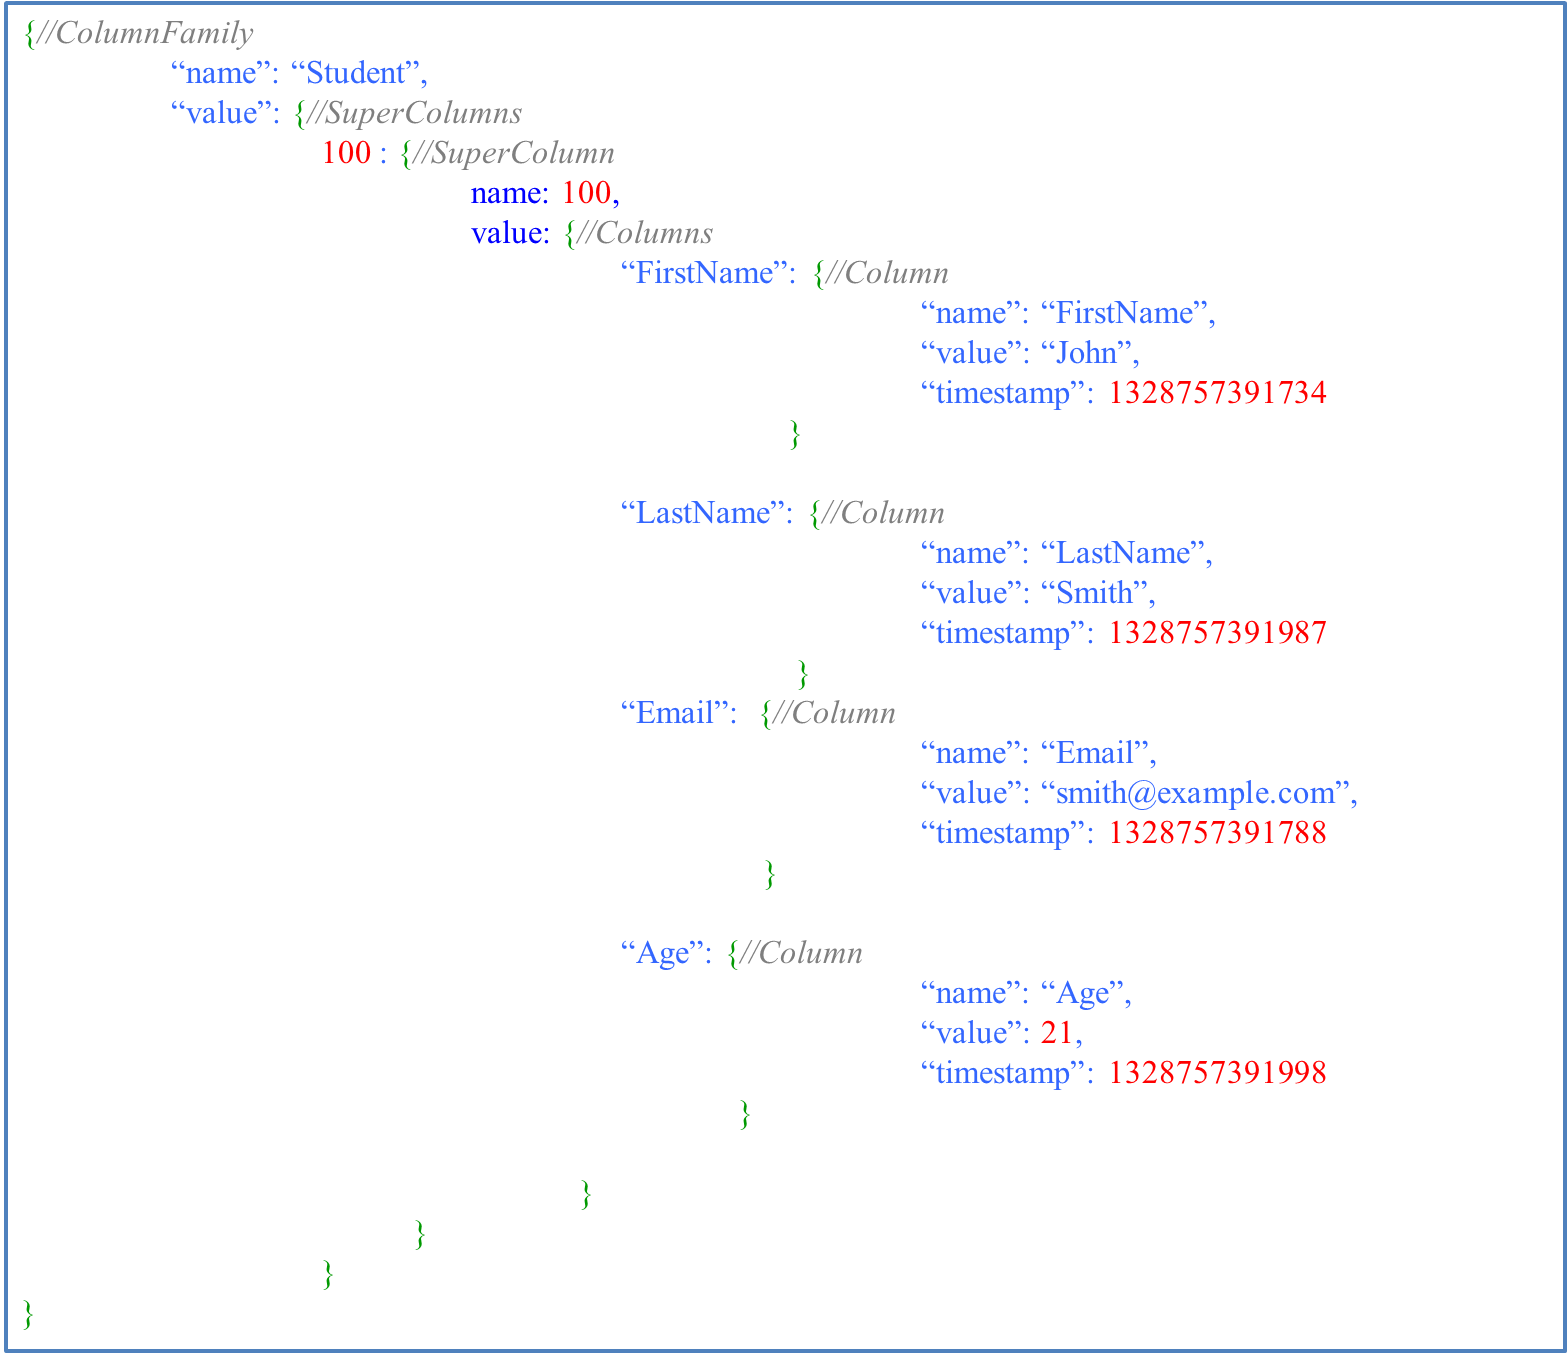
\includegraphics[width=\textwidth]{./figure/Example/JSON_ColumnFamily_1row.png}
	\caption{JSON notation for a column family in
	Cassandra}\label{f:columnfamilyJSON}
\end{figure} 

\subsection{KeySpace}
 A keyspace is a container to hold the data that the
application uses.  Keyspaces have one or more column families,   although it is not strictly
required that a keyspace should always have column families.  Any relationships
existing between column families in a keyspace are not preserved. 

A keyspace can be considered similar to a database in traditional relational
databases,   without any relationships.  An example of the keyspace
University is shown in Figure~\ref{f:keyspace}. 

Keyspaces require that some attributes are defined,   like a user defined name,  
replication strategy and others.  Some optional elements that can be defined are
the details of the column families in the keyspace and other options
for replication of data. 
% \end{description}
 
%\newpage



\begin{landscape}
\begin{figure}[h]
	\centering
	%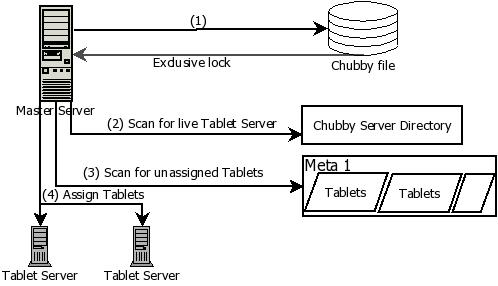
\includegraphics[width=5cm,   height=5cm]{. /figure/random. jpg}
	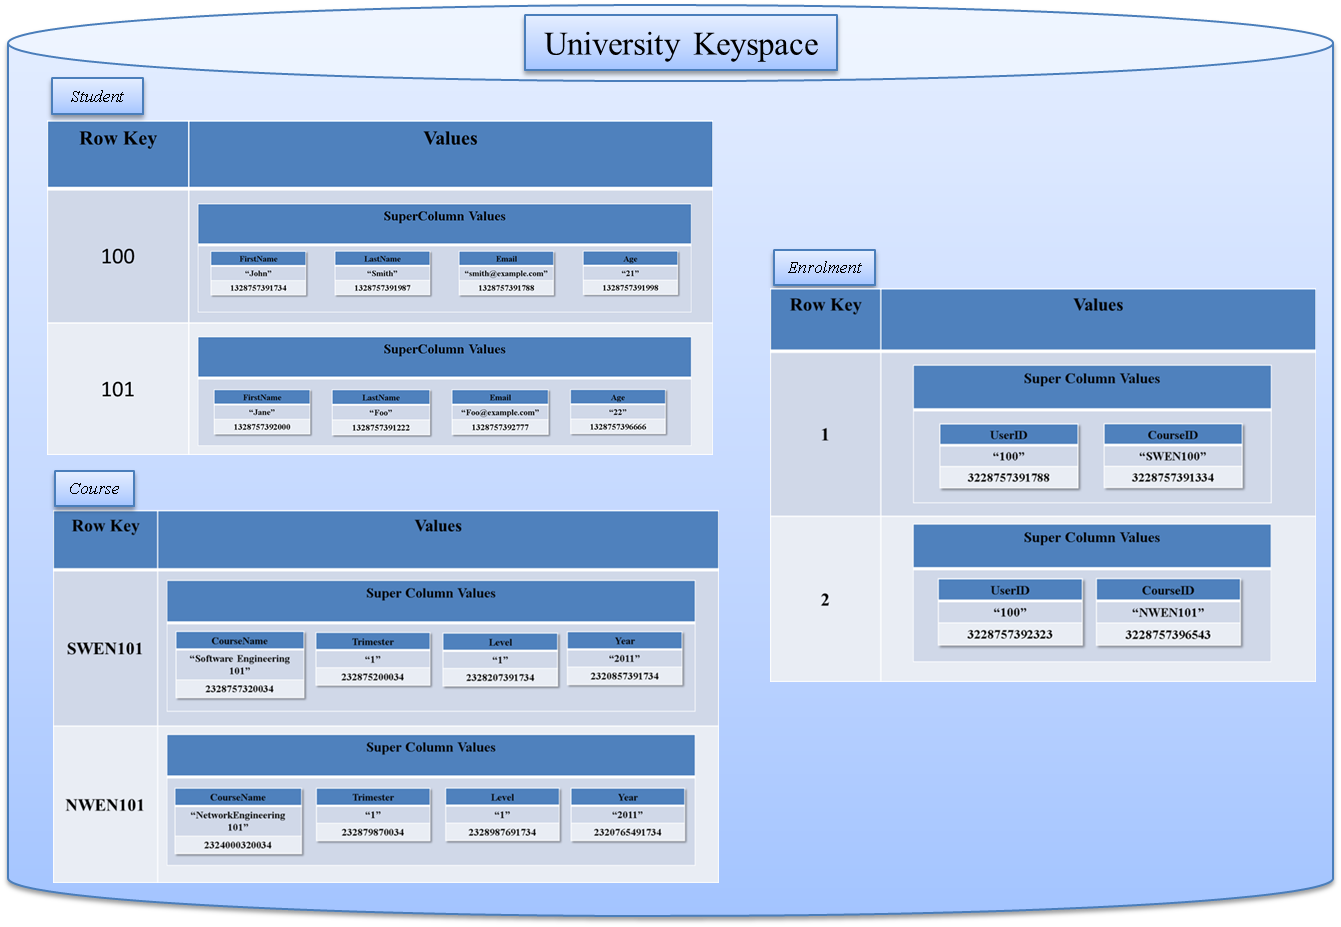
\includegraphics[width=1.4\textwidth]{./figure/Example/KEYSPACE.png}
	\caption{A keyspace in
	Cassandra}\label{f:keyspace}
\end{figure}
\end{landscape}
